\chapter{Wstęp}



\section{Opis problemu}\label{ch:wstep}

\par Motywacją powstania projektu były zawodowe doświadczenia członków zespołu projektowego. Podczas pracy ze sprzętem komputerowym, na różnorodnych stanowiskach, elementem łączącym wszystkie te stanowiska był brak odpowiedniego oprogramowania do efektywnego zarządzania oraz monitorowania infrastruktury sprzętowej w jednym, scentralizowanym systemie łączącym funkcje ewidencji sprzętu z telemetrią.
\par Z tego względu zespół projektowy podjął się stworzenia systemu \gls{open-source} przyjaznego użytkownikowi zarówno w obsłudze, utrzymaniu jak i wdrożeniu co ma zachęcić i przekonać organizacje do używania podobnych rozwiązań.
\begin{figure}[H]
    \centering
    \caption{Rich Picture}
    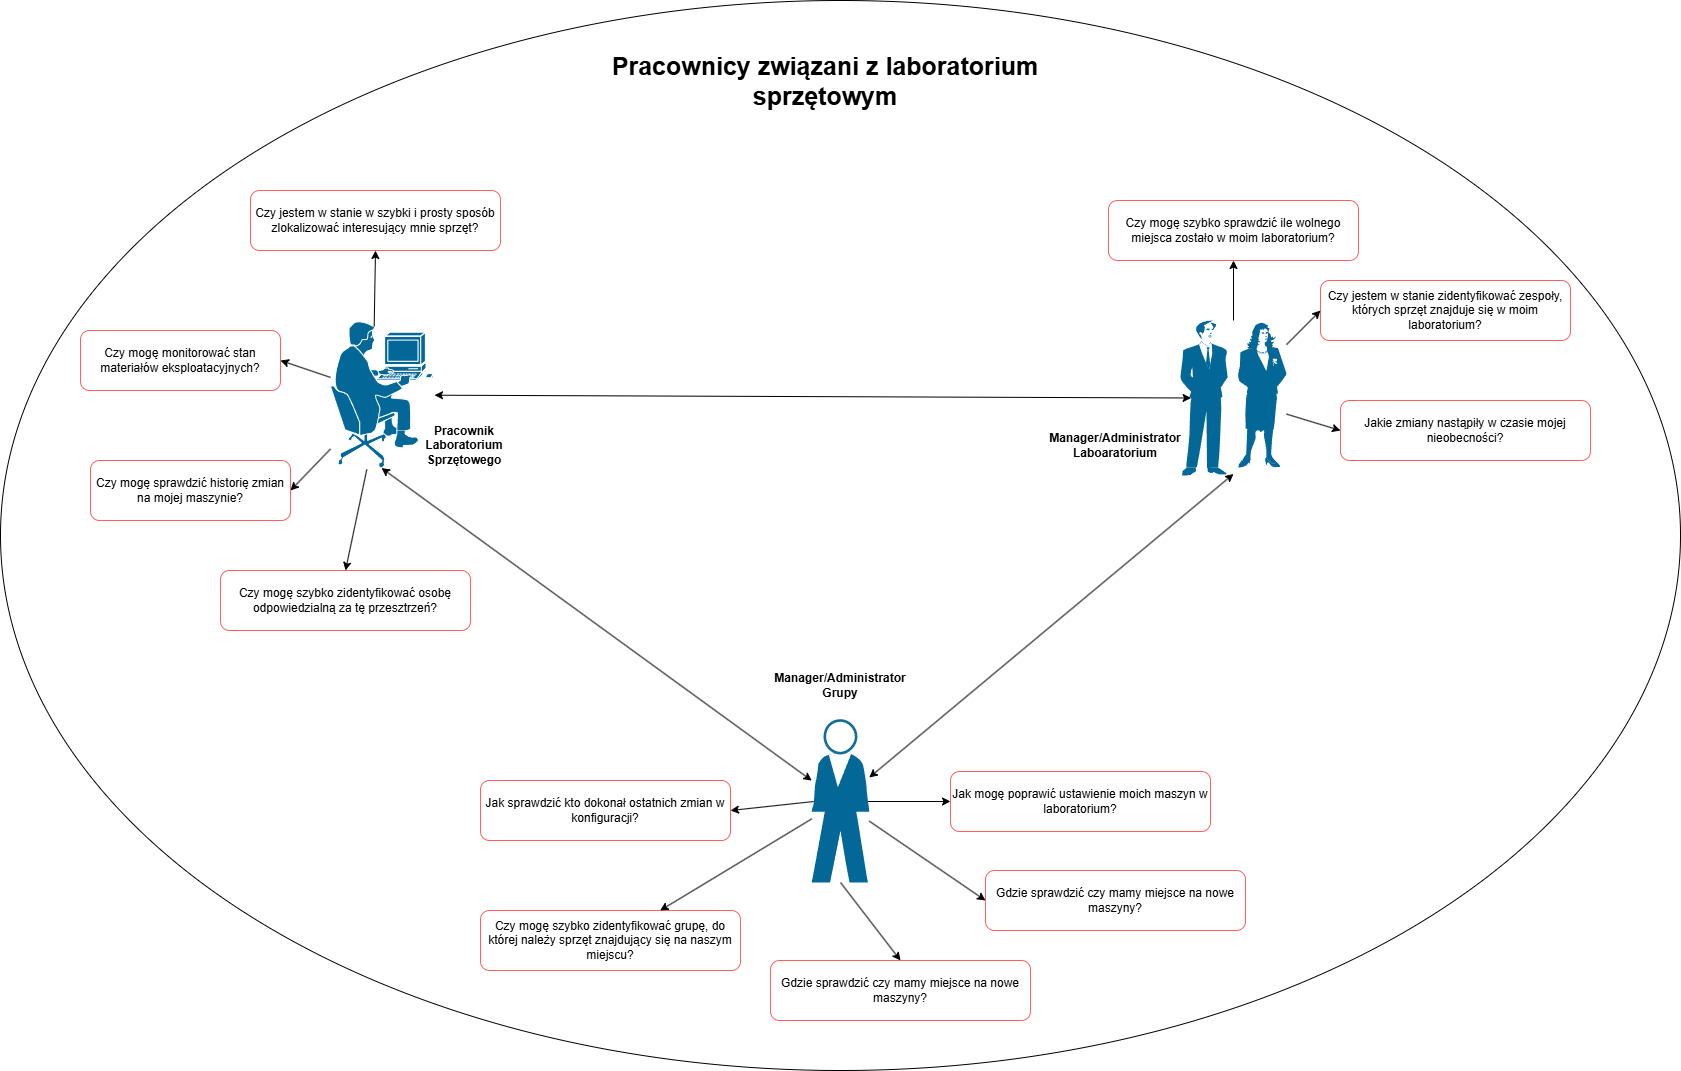
\includegraphics[width=1.0\textwidth]{images/diagramy/rich_picture.png} 
    \caption*{Źródło: Opracowanie własne}
    \label{img:rich_picture}
\end{figure}


\section{Przegląd istniejących rozwiązań}
\par Na rynku dostępny jest szereg gotowych rozwiązań problemu postawionego w tej pracy inżynierskiej. Większość z nich jest płatna oraz opiera się na przetrzymywaniu danych w chmurze, a nie lokalnie co dla wielu organizacji jest kolejnym potencjalnym ryzykiem, na które nie mogą sobie pozwolić. Przykładowe rozwiązania:
\begin{itemize}
    \item \textbf{RackTables} \url{https://www.racktables.org}
    \item \textbf{Nautobot} \url{https://networktocode.com/nautobot/}
    \item \textbf{Device42} \url{https://www.device42.com}
\end{itemize}

Podobnym projektem jest produkt firmy NetBox Labs, Inc. Jest on niewątpliwie rozwiązaniem konkurencyjnym pod względem funkcjonalności jakie oferuje. Umożliwia ono szereg funkcji od zarządzania \gls{platforma}mi, połączeniami sieciowymi po rozproszony system kontroli wersji z możliwością działania w pełni w chmurze. Jest to system wiele bardziej zaawansowany od zaprojektowanego w ramach tej pracy dyplomowej, jednak jest on systemem płatnym, posiadającym bardzo okrojone darmowe wersje, a także wymagającym skomplikowanego planowania jak i wdrożenia.
Potwierdzenie tego stanu rzeczy możemy zauważyć na forach dyskusyjnych:
\begin{quote}
    \item "Is there an easier way to install netbox?" (tłum. własne: "Czy jest łatwiejszy sposób na zainstalowanie netbox?") - Użytkownik Esctatic\_Orange66, Reddit \cite{netbox_newbie}
\end{quote}
\begin{quote}
    \item "I am installing a new netbox V4.4.4 and i am stuck at the last step(...)" (tłum. własne: "Instaluję nowego netbox'a V4.4.4 i utknąłem na ostatnim kroku") - Użytkownik doc\_doggo, Reddit \cite{netbox_stuck}
\end{quote}
W przeciwieństwie do naszego rozwiązania nie posiada on również mapy przestrzennej \gls{laboratorium}.

\section{Proponowane rozwiązanie}
\par Celem realizacji projektu, jest stworzenie systemu zarządzania i monitorowania inwentarzem technicznym, który będzie w stanie sprostać podstawowym potrzebom w pracy ze sprzętem komputerowym. Cel pracy został ograniczony do kluczowych funkcjonalności systemu ze względu na ograniczenia projektowe. Oprogramowanie celowane jest do organizacji bez podobnego rozwiązania zatem wdrożenie systemu musi być proste oraz pozwolić w łatwy sposób przenieść aktualnie kompletowane dane. Cechą kluczową systemu jest mapa przestrzenna \gls{laboratorium}, która oprócz zwiększenia efektywności prac, ułatwia proces \gls{onboarding}'u pozwalając zapoznać się z zasobami organizacji w sposób zorganizowany z ułatwionym i zcentralizowanym dostępem do informacji.